\secput{results}{Results}
We implemented each of the simple solutions described in 
\secref{simple}, and compared their performance to range coalescing on a variety of data sets. 

Range coalescing performs significantly better in practice than other 
linear-storage solutions. It performs better on both small and large datasets. 
As the datasets get larger, the effects of range coalescing become more evident. 
For $n=50$ and $k=1000$, range coalescing does 5 times better than a simple binary search,
whereas for $n=5000$ and $k=1000$, range coalescing performs 18 times better.

However, range coalescing requires much more time for initialization. 
It takes about 20 times longer than initialize than the vEB search. 
We believe these results could be improved upon, but we leave that as future work.

We implemented a full merge, not the randomized solution...

What about setup time for fractional cascading and quadratic?




\begin{figure}
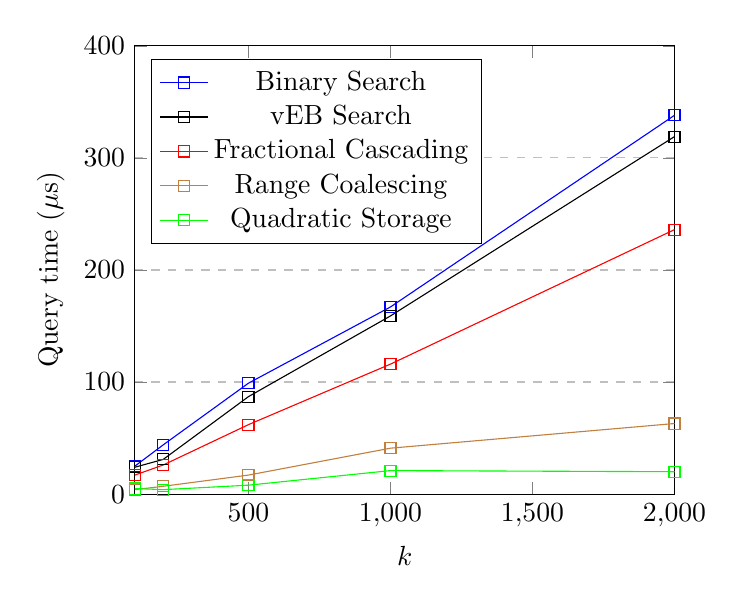
\begin{tikzpicture}
\begin{axis}[
    %title={},
    xlabel={$k$},
    ylabel={Query time ($\mu$s)},
    xmin=100, xmax=2000,
    ymin=0, ymax=400,
    legend pos=north west,
    ymajorgrids=true,
    grid style=dashed,
]
 
  \addplot[color=blue,mark=square] coordinates {(100,25)(200,44)(500,99)(1000,167)(2000,338)};
    \addlegendentry{Binary Search}
 
  \addplot[color=black,mark=square] coordinates {(100, 24) (200, 31) (500,87)(1000,159)(2000,319)};
    \addlegendentry{vEB Search};

  \addplot[color=red,mark=square] coordinates {(100, 17) (200, 26)(500,62)(1000,116)(2000,236)};
    \addlegendentry{Fractional Cascading}

  \addplot[color=brown,mark=square] coordinates {(100, 4) (200, 7)(500,17)(1000,41)(2000,63)};
    \addlegendentry{Range Coalescing};
  \addplot[color=green,mark=square] coordinates {(100, 5) (200, 4)(500,8)(1000,21)(2000,20)};
    \addlegendentry{Quadratic Storage};
\end{axis}
\end{tikzpicture}
\caption{Query times vs $k$ (for fixed $n$=1000).  SNARF: details on experimental setup.}
\end{figure}

\begin{figure}
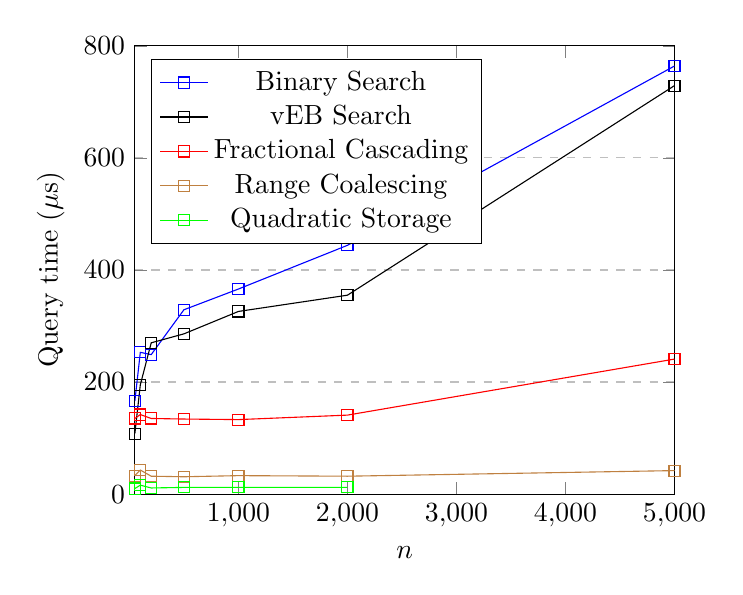
\begin{tikzpicture}
\begin{axis}[
    %title={},
    xlabel={$n$},
    ylabel={Query time ($\mu$s)},
    xmin=50, xmax=5000,
    ymin=0, ymax=800,
    legend pos=north west,
    ymajorgrids=true,
    grid style=dashed,
]
 
  \addplot[color=blue,mark=square] coordinates {(50,166)(100,253)(200,249)(500,329)(1000,366)(2000,444)(5000,764)};
    \addlegendentry{Binary Search}
 
  \addplot[color=black,mark=square] coordinates {(50,108)(100,195)(200,270)(500,286)(1000,326)(2000,355)(5000,729)};
    \addlegendentry{vEB Search};

  \addplot[color=red,mark=square] coordinates {(50,135)(100,142)(200,135)(500,134)(1000,133)(2000,141)(5000,241)};
    \addlegendentry{Fractional Cascading}

  \addplot[color=brown,mark=square] coordinates {(50,33)(100,43)(200,32)(500,31)(1000,33)(2000,32)(5000,42)};
    \addlegendentry{Range Coalescing};
  \addplot[color=green,mark=square] coordinates {(50,10)(100,16)(200,11)(500,12)(1000,12)(2000,12)};
    \addlegendentry{Quadratic Storage};
\end{axis}
\end{tikzpicture}
\caption{Query times vs $n$ (for fixed $k$=1000).  SNARF: details on experimental setup.}
\end{figure}
